\chapter{Comptage variationnel quantique}
\label{cha:comptage-variationnel-quantique}

%-----------------------------------------------------------------------------%

Les chapitres précédents ont laissé transparaître l'intuition derrière l'approche empruntée dans ce travail: est-il possible d'utiliser les algorithmes variationnels quantiques comme générateur de solutions à l'algorithme de JVV pour la résolution approximative des problèmes de comptage? Avant d'introduire le fruit du travail de ce mémoire, l'algorithme VQCount, énumérons les difficultés liées à la résolution de problèmes de comptage avec les algorithmes variationnels quantiques. D'abord, les circuits quantiques doivent produire une grande séparation entre les amplitudes des solutions et les non-solutions de l'état produit pour pouvoir produire même une seule solution avec un nombre tractable de mesures. Ensuite, même si les amplitudes des non-solutions sont nulles, si les amplitudes d'un sous-ensemble non négligeable des solutions sont significativement supprimées par rapport aux autres amplitudes, la mesure des états supprimés entraîne une surcharge computationnelle, potentiellement exponentielle, du nombre de répétitions. Finalement, même si toutes les solutions possèdent environ des amplitudes égales et si les non-solutions ne sont pas présentes dans l'état produit, un nombre exponentiel de mesures est en théorie nécessaire pour énumérer naïvement les solutions de manière exhaustive, comme le nombre de solutions est exponentiel pour les problèmes d'intérêt.

L'apport principal de ce travail réside dans la combinaison des algorithmes variationnels quantique et l'algorithme de JVV. L'algorithme VQCount échantillonne la distribution préparée par GM-QAOA afin de produire un compte approximatif à l'aide de l'algorithme de JVV. Cette approche tente de minimiser l'impact des obstacles précédents, en particulier de la deuxième et troisième difficulté. L'utilisation de GM-QAOA permet d'éviter la suppression d'amplitude d'un sous-ensemble de solutions en assurant que toutes les solutions aient la même amplitude. De plus, l'algorithme de JVV tire avantage de la structure des problèmes auto-réductibles pour éviter de devoir énumérer naïvement toutes les solutions. Afin de prendre en compte la propriété d'auto-réductibilité, le circuit GM-QAOA doit nécessairement être modifié. Une procédure d'auto-réduction, comprise dans l'algorithme VQCount, modifie ainsi itérativement le circuit pour la résolution des sous-problèmes tout en conservant les propriétés de GM-QAOA.

Ce chapitre débute en introduisant l'algorithme VQCount à la section~\ref{sec:algorithme-vqcount} et décrit la procédure d'auto-réduction nécessaire à l'algorithme VQCount à la section~\ref{sec:procedure-auto-reduction}.

%-----------------------------------------------------------------------------%

\section{Algorithme VQCount}
\label{sec:algorithme-vqcount}

Comment faire le pont entre les algorithmes variationnels quantiques et l'algorithme de JVV pour la résolution de problème de comptage? A priori, l'algorithme de JVV doit tout simplement être implémenté en utilisant un algorithme variationnel quantique comme générateur de solutions. Cependant, plusieurs embûches barrent notre chemin. Décrivons la procédure, nommée VQCount par brièveté, en affrontant ces problèmes en chemin.

Soit une instance de problème SAT, décrite par la formule CNF $\varphi$. Ce problème est auto-réductible par la relation~\ref{rel:auto-reductibilite-sat}. Ce travail se limite à l'étude du problème SAT en gardant en tête que, par sa \textsf{NP}-complétude, une réduction existe entre n'importe quel problème de la classe \textsf{NP} et celui-ci. La formule $\varphi$ peut être transformée en un modèle d'Ising, tel que décrit à la section~\ref{subsec:encodage-probleme}, de sorte que l'hamiltonien du modèle d'Ising $H_{P}$ encode le problème. Grâce à cet hamiltonien de problème, le circuit paramétré quantique de l'algorithme QAOA est construit en préparant l'état $\ket{\psi(\vec{\gamma}_{0}, \vec{\beta}_{0})}$ avec les paramètres initiaux $\vec{\gamma}_0$ et $\vec{\beta}_{0}$. Négligeons pour le moment le choix de l'état initial et de l'hamiltonien de forçage. Une fois le circuit construit, l'énergie moyenne de $H_{P}$ est évaluée à l'aide de mesures répétées de l'état préparé. Un optimiseur classique modifie ensuite les paramètres du circuit quantique pour minimiser cette énergie, donnant un circuit quantique paramétré optimisé $\ket{\psi(\vec{\gamma}, \vec{\beta})}$.
Les échantillons, obtenus par des mesures de l'état préparé par le circuit dans la base computationnelle, contiennent alors des solutions à la formule $\varphi$ avec une haute probabilité.

QAOA étant une méthode heuristique, les paramètres optimaux ne sont pas nécessairement atteints, impliquant la présence de non-solutions dans la distribution obtenue en mesurant $\ket{\psi(\vec{\gamma}, \vec{\beta})}$. L'algorithme de JVV nécessite pourtant une distribution composée uniquement de solutions, impliquant qu'une étape de post-traitement doit être employée pour retirer les non-solutions. Comme le problème SAT appartient à la classe \textsf{NP}, vérifier qu'un échantillon est une solution est un processus efficace. Ainsi, toutes les non-solutions échantillonnées sont retirées de la distribution obtenue. De plus, comme discuté à la section~\ref{sec:echantillonnage-et-biais}, la non-uniformité de la distribution obtenue ne respecte pas nécessairement la condition de l'algorithme de JVV. La discussion dans cette section se restreint alors à la variante GM-QAOA, qui garantit que les amplitudes des solutions préparées soient égales. Ainsi, le critère de mérite pertinent est la probabilité que le résultat d'une mesure soit une solution, ou plus succinctement le \textit{taux de succès}
\begin{equation}
    r = \braket{ \psi(\vec{\gamma}, \vec{\beta}) | \hat{\mathcal{P}}_{G} | \psi(\vec{\gamma}, \vec{\beta}) } \,,
\end{equation}
où $\hat{\mathcal{P}}_{G}$ est le projecteur dans l'espace des solutions $G$, c'est-à-dire l'état fondamental du modèle d'Ising représentant le problème, donné par
\begin{equation}
    \hat{\mathcal{P}}_{G} = \sum_{x \in G} \ket{x}\!\bra{x} \,.
\end{equation}
Cette définition permet alors de décrire la performance des différents algorithmes pour le comptage basé sur l'échantillonnage sur un pied d'égalité en utilisant le taux de succès $r$, la tolérance (ou l'erreur multiplicative) $\varepsilon$ ainsi que la confiance $\delta$. Cette caractérisation s'étend aux algorithmes classiques employant un générateur échouant à produire une solution à un taux $1 - r$.

Ces remarques complétées, des échantillons sont mesurés à partir du circuit $\ket{\vec{\gamma}, \vec{\beta}}$ pour estimer la valeur la plus probable $w_{1}$ de la première variable $x_{1}$. Selon l'algorithme de JVV, il faut alors échantillonner des solutions à la sous-instance $\varphi_{w_{1}}$. Résoudre directement celle-ci à l'aide du même circuit optimisé demanderait une post-sélection supplémentaire sur la première variable. En réalité, comme il existe un nombre exponentiel de sous-instances en raison du nombre exponentiel de chaînes de bits possibles, un nombre exponentiel d'échantillons supplémentaires devraient être échantillonnés. Une autre méthode consiste à construire et optimiser un différent circuit pour résoudre la sous-instance. Pour éviter cette surcharge computationnelle, le circuit de GM-QAOA est modifié pour résoudre directement la sous-instance. Cette procédure, nommée procédure d'auto-réduction, consiste à remplacer, pour chaque qubit fixé, la porte d'Hadamard par une porte de Pauli conditionnée sur la valeur $w_{0}$ du bit fixé et à retirer la composante de l'opérateur de forçage sur le qubit associé. Cette procédure est détaillée à la section~\ref{sec:procedure-auto-reduction}. Ce changement permet de conserver la propriété d'égalité des amplitudes de GM-QAOA. De plus, celle-ci suggère qu'il soit possible d'éviter d'optimiser à nouveau le circuit en gardant les mêmes paramètres. Ainsi, le circuit est modifié selon la procédure d'auto-réduction sans procéder à une nouvelle ronde d'optimisation. Des solutions sont alors encore échantillonnées de ce sous-circuit et le processus est répété de manière récursive jusqu'à ce que toutes les variables soient fixées. Le nombre de solutions est alors donné par l'inverse du produit des probabilités conditionnelles tel qu'énoncé par l'algorithme de JVV. L'algorithme~\ref{alg:algorithme-jvv} résume les étapes de l'algorithme VQCount.

\begin{algorithm}[ht!]
    \caption{VQCount}\label{alg:vqcount}
    \begin{algorithmic}[1]
    \REQUIRE Nombre de variables: $n$, Hamiltonien de problème: $H_P$,\\Hamiltonien de forçage: $H_D$, Paramètres initiaux: $(\vec{\gamma}_0, \vec{\beta}_0)$, Profondeur: $p$, Nombre d'étapes d'optimisation: $n_{o}$, Nombre de solutions à\\échantillonner: $n_s$
    \STATE PQC($\vec{\gamma}_0, \vec{\beta}_0) \leftarrow \text{Circuit-QAOA}(H_P, H_D, \vec{\gamma}_0, \vec{\beta}_0, p$) \\
    \COMMENT{PQC : Circuit quantique paramétré}
    \STATE $\text{PQC}(\vec{\gamma}, \vec{\beta}) \leftarrow \text{Optimisation}(\text{PQC}(\vec{\gamma}_0, \vec{\beta}_0), n_{o})$
    \STATE $\tilde{N} \leftarrow 1$
    \FOR{$i \in \{1, \dots, n\}$}
    \STATE $S \leftarrow \{ \ \}$
    \WHILE{$\abs{S} < n_{s}$}
    \STATE $m \leftarrow \text{Mesure}(\text{PQC}(\vec{\gamma}, \vec{\beta}))$
    \IF{$\text{Vérification-Solution}(m, H_{P})$}
    \STATE $S \leftarrow S \cup \{m\}$
    \ENDIF
    \ENDWHILE
    \STATE $w, \tilde{p} \leftarrow \text{Préfixe-Majoritaire}(S)$
    \STATE $\text{PQC}(\vec{\gamma}, \vec{\beta}) \leftarrow \text{Auto-Réduction}(\text{PQC}(\vec{\gamma}, \vec{\beta}), w)$
    \STATE $\tilde{N} \leftarrow \tilde{N} / \tilde{p}$
    \ENDFOR
    \RETURN $\tilde{N}$
\end{algorithmic}
\end{algorithm}
    
Comme l'algorithme VQCount se base sur celui de JVV, son utilisation requiert $O(\frac{n^{2} \log (\delta^{-1})}{r \varepsilon^{2}})$ échantillons pour estimer le nombre d'états fondamentaux à une erreur multiplicative $\varepsilon$ avec une confiance $1 - \delta$ pour un taux de succès $r$. Ce résultat se compare favorablement à un travail similaire évaluant la fonction de partition d'hamiltoniens de spins classiques qui nécessite $O(\frac{\sqrt{N \log(\delta^{-1})}}{r \varepsilon})$ échantillons pour la même tâche~\cite{sundarQuantumAlgorithmCount2019}. Lorsque $N=O(2^{n})$, VQCount nécessite exponentiellement moins d'échantillons que cette méthode. Notons qu'un algorithme classique peut être utilisé pour résoudre l'instance du problème de comptage lorsque VQCount a suffisamment réduit celle-ci.

Bien que l'approche présentée règle certains des problèmes énoncés au début de la section, les problèmes \textsf{\#P}-difficile demeurent difficiles pour les ordinateurs quantiques. La génération des distributions arbitraires, incluant les distributions uniformes de structures combinatoires, est difficile en général et seulement facile dans des cas exceptionnels~\cite{aaronsonComputationalComplexityLinear2011, boulandComplexityVerificationQuantum2019}. De plus, GM-QAOA requiert en général des profondeurs de circuits de taille exponentielle selon la taille du problème pour atteindre un taux de succès fini~\cite{xiePerformanceUpperBound2025}. 

%-----------------------------------------------------------------------------%

\section{Procédure d'auto-réduction}
\label{sec:procedure-auto-reduction}

Pour agir en tant que générateur de solutions à la sous-instance de l'instance du problème original, le circuit GM-QAOA doit être modifié pour être en mesure d'échantillonner à partir de la distribution de solutions appropriée. Comme expliqué à la section précédente, il n'est pas suffisant d'échantillonner l'état produit par le circuit original en raison du nombre exponentiel de mesures supplémentaires nécessaires. Une \textit{procédure d'auto-réduction}, illustrée à la figure~\ref{fig:vqcount-circuit}, est alors introduite pour résoudre cette complication. Soit une formule CNF $\varphi$ de taille $n$ et une sous-formule CNF $\varphi_{w}$ représentant la formule $\varphi$ où les premières variables sont remplacées par $w$. Alors, pour chaque qubit $q$ fixé à $\ket{w_{q}}$ du circuit GM-QAOA, les opérations suivantes sont appliquées:

\begin{enumerate}[(1)]
    \item Retirer la porte d'Hadamard $H$ initiale du qubit $q$.
    \item Insérer un porte de Pauli $X$ classiquement conditionnée par la valeur $w_{q}$.
    \item Retirer l'opérateur de l'hamiltonien de forçage $H_{D}$ du qubit $q$.
\end{enumerate}

Ces modifications fixent alors l'état du qubit $q$ à $\ket{w_{q}}$ tout en préservant les termes d'interactions encodant les contraintes de la formule $\varphi_{w}$. Comme l'opérateur de forçage $U_{D}$ n'est plus appliqué au qubit $q$, celui-ci demeure dans le même état, à une phase près, spécifié par la porte de Pauli $X$. En effet, l'opérateur de problème n'applique qu'une phase globale sur le qubit $q$. Le sous-circuit, c'est-à-dire le circuit initial sans le qubit $q$, résout alors le sous-problème tout en conservant les mêmes propriétés de GM-QAOA. En effet, similairement à propriété d'auto-réductibilité du problème SAT, le modèle d'Ising est aussi auto-réductible. Considérons un terme d'interaction $Z_{q}Z_{p}$ de ce modèle appliqué sur les spins $q$ et $p$. Fixer le spin $q$ à une valeur constante $\sigma_{q}$ signifie que l'influence de ce terme sur le spin $p$ peut être vu comme un terme de champ magnétique local $\sigma_{q} Z_{p}$. Le sous-circuit peut ainsi être reconstruit en tirant avantage de la propriété d'auto-réductibilité du modèle d'Ising. Avec cette perspective, nous remarquons que le sous-circuit constitue aussi un circuit GM-QAOA.     

\begin{figure}[h]
    \centering
    \begin{subfigure}[h]{0.7\textwidth}
        \centering
        \caption{}
        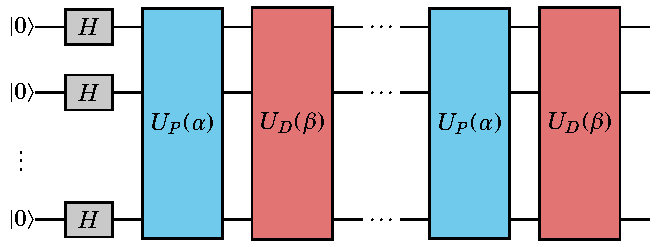
\includegraphics[width=1\textwidth]{figures/qaoa-self-reducibility-1.pdf}
        \label{fig:vqcount-circuit-a}
    \end{subfigure}
    \begin{subfigure}[h]{0.7\textwidth}
        \centering
        \caption{}
        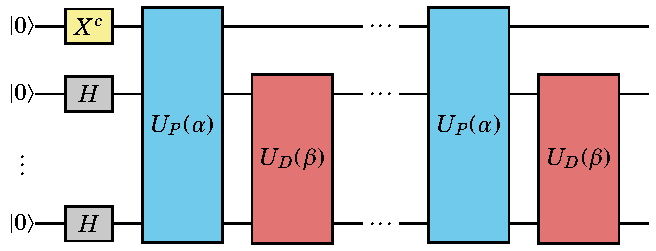
\includegraphics[width=1\textwidth]{figures/qaoa-self-reducibility-2.pdf}
        \label{fig:vqcount-circuit-b}
    \end{subfigure}
    \caption[Procédure d'auto-réduction de VQCount]{Générateur de solutions QAOA avant (a) et après (b) avoir fixé le premier qubit à $c$ durant la procédure d'auto-réduction. La porte d'Hadamard $H$ agissant sur le qubit fixé est remplacée par la porte de Pauli-X, conditionnée classiquement sur $c$. Pour chaque couche, l'opérateur de problème $U_{P}(\gamma)$ reste inchangé, tandis que les portes de l'opérateur de forçage $U_{D}(\beta)$ agissant sur le qubit fixé sont retirées.}
    \label{fig:vqcount-circuit} 
\end{figure}

Le développement de cette procédure a aussi mené à une expression récursive fermée de l'état préparé par le circuit GM-QAOA, présenté dans l'annexe~\ref{ann:expression-fermee-etat-circuit-gm-qaoa}.

L'algorithme VQCount ne comprend qu'une optimisation des paramètres du circuit quantique paramétré avant la procédure d'auto-réduction. Toutefois, un autre cycle d'optimisation est en principe nécessaire pour chaque circuit réduit afin d'atteindre un état optimal représentant les solutions à la sous-instance du problème. Ce choix mène alors à la question suivante: est-ce que la probabilité de succès $r$ du circuit réduit est égale ou supérieure à celle du circuit original avec les mêmes paramètres? Dans ce cas, l'optimisation n'est nécessaire que pour le circuit original et peut être évitée pour les circuits réduits.

La réponse à cette question est positive pour les circuits GM-QAOA dans la limite $\gamma_{i}=\beta_{i}$, $i=1,\dots,p$. Dans cette limite, GM-QAOA se réduit à l'algorithme de Grover. En effet, comme décrit ci-dessous, pour tous les hamiltoniens de problème $H_{P}$ pouvant être écrit comme une somme de chaînes de Pauli, un circuit peut être construit pour effondrer tous les niveaux excités de $H_{P}$ à un seul niveau excité, ce qui donne un hamiltonien d'évolution à deux niveaux $H_{P}$. Avec les paramètres susmentionnés, l'opérateur de problème $U_{P}$ devient un oracle pour les états fondamentaux de $H_{P}$, à une phase constante près, et $U_{D}$ devient l'opérateur de diffusion de Grover. Dans cette limite, à une profondeur constante $p=O(1)$, le taux de succès est une fonction strictement croissante du rapport des solutions au nombre total d'états. Si, en descendant l'arbre d'auto-réductibilité de l'algorithme de JVV, nous choisissons les branches possédant une probabilité plus grande que $1/2$, alors le ratio des solutions au nombre total d'états est aussi strictement croissant. Cela signifie que, pour ce choix de paramètres, un circuit GM-QAOA pour un problème donné peut être modifié selon la procédure d'auto-réduction pour résoudre les sous-problèmes avec le même ou un meilleur taux de succès. Cet argument est seulement valide dans la limite de Grover, mais suggère que la stratégie d'auto-réduction est possiblement aussi valide dans d'autres cas. Le chapitre suivant introduit des évidences sous la forme de simulations numériques pour confirmer la validité de cette intuition.

Comment est-il possible d'effondrer une multitude de niveaux excités à un unique niveau excité pour un hamiltonien $H_{P}$ à l'aide d'un circuit? Montrons un exemple avec le circuit illustré à la figure~\ref{fig:tower-excited-states-circuit}. Ce circuit effondre les états excités pour un problème NAE3SAT décrit par la formule CNF $\varphi = (x_{1} \lor x_{2} \lor x_{3}) \land (x_{4} \lor x_{5} \lor x_{6})$. Le premier registre du circuit, composé de trois qubits d'entrées, deux qubits de parité et un qubit de contrôle, concerne la première clause. De même, un deuxième registre, identique au premier registre, concerne la deuxième clause. Le dernier qubit de phase s'occupe de l'application d'une phase aux solutions.

Pour comprendre ce circuit, déterminons d'abord l'état des qubits du premier registre juste avant l'application de l'opérateur de phase multicontrôlé $Z^{-\gamma \pi}$. Les qubits d'entrées correspondent aux valeurs prises par les littéraux de la première clause de $\varphi$. La parité des couples de littéraux $(x_{1}, x_{2})$ et $(x_{2}, x_{3})$ de cette clause est d'abord sauvegardée dans les deux qubits de parité à l'aide de portes CNOT. Par la suite, une porte NOT est appliquée sur les qubits de parité. Finalement, une porte de Toffoli transforme le qubit de contrôle si l'état des qubits de parité est $\ket{11}$. Le tableau~\ref{tab:tower-excited-states-parity} présente les valeurs des qubits mentionnés selon les différentes valeurs des qubits d'entrée à ce point du circuit.

\begin{table}[ht!]
    \centering
    \begin{tabular}{c c c}
        \hline
        Entrée & Parité & Contrôle \\
        \hline
        000 & 11 & 1 \\
        001 & 10 & 0 \\
        010 & 00 & 0 \\
        100 & 01 & 0 \\
        011 & 01 & 0 \\
        101 & 00 & 0 \\
        110 & 10 & 0 \\
        111 & 11 & 1 \\
        \hline
    \end{tabular}
    \caption{État des différents qubits du premier registre du circuit d'effondrement des états excités avant l'application de l'opérateur de phase $Z^{-\gamma \varepsilon \pi}$.}
    \label{tab:tower-excited-states-parity}
\end{table}

Remarquons que le qubit de contrôle est dans l'état $\ket{1}$ seulement si les qubits d'entrée sont dans l'état $\ket{000}$ ou $\ket{111}$, c'est-à-dire les non-solutions du problème NAE3SAT. Le qubit de contrôle indique donc si une clause est satisfaite ou insatisfaite. Cette procédure s'applique aussi au deuxième registre, où le qubit de contrôle de celui-ci indique si la deuxième clause est respectée. Sachant cela, un opérateur de phase $Z^{-\gamma \varepsilon \pi}$ anti-contrôlé sur tous les qubits de contrôle permet d'appliquer une phase $e^{-i \gamma \varepsilon}$ uniquement aux solutions. Après l'application de cette phase, l'inverse du circuit est appliqué pour rétablir l'état initial~\cite{nielsenQuantumComputationQuantum2011}.

\begin{figure}[ht!]
    \centering
    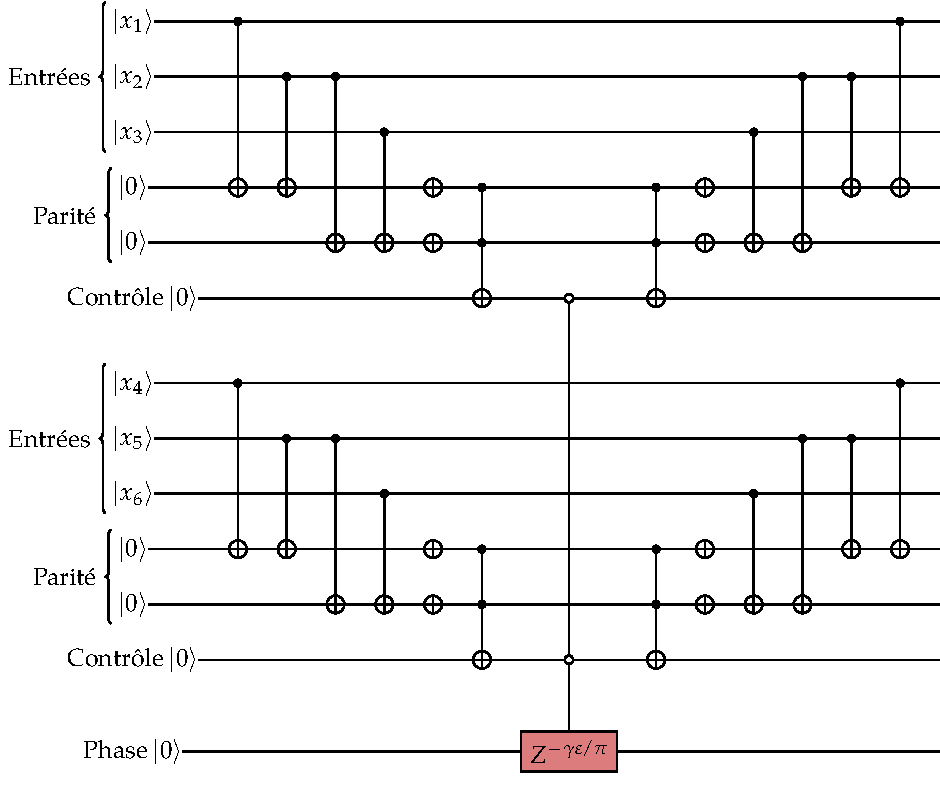
\includegraphics[width=1\textwidth]{figures/tower-excited-states-circuit.pdf}
    \caption[Circuit d'effondrement des états excités]{Exemple d'un circuit d'effondrement des états excités. Pour une formule CNF $\varphi = (x_{1} \lor x_{2} \lor x_{3}) \land (x_{4} \lor x_{5} \lor x_{6})$ décrivant un problème NAE3SAT, ce circuit applique l'opérateur $Z^{-\gamma \varepsilon / \pi}$ uniquement aux solutions du problème.}
    \label{fig:tower-excited-states-circuit}
\end{figure}

